\section{Compiler}
\subsection{Grammar Engineering}
\subsubsection{First sets}
$First(X)$ bestimmen:
\begin{enumerate}
	\item Falls $X$ Terminal: $First(X) = \{X\}$
	\item Falls $X  \rightarrow \epsilon$ füge $\epsilon$ zu $First(X)$
	\item Falls $X \rightarrow Y_1..Y_n$ füge $First(Y_1..Y_n)$ zu $First(X)$
	\item $First(Y_1..Y_n)$ ist entweder
	\begin{enumerate}
		\item $First(Y_1)$, iff $Y_1  \nrightarrow \epsilon$
		\item $First(Y_1) \backslash \{\epsilon\} \cup First(Y_2..Y_n)$,  falls $\exists k \in [2,n]: Y_k \nrightarrow \epsilon$
		\item rekursiv fortführen
	\end{enumerate}
\end{enumerate}
\subsubsection{Follow sets}
$Follow(X)$ bestimmen:
\begin{enumerate}
	\item Füge $\#$ zu $Follow(X)$, falls $X=S$
	\item Falls $A \rightarrow aXb$ und $\epsilon \centernot\in First(b)$, dann füge $First(b)$ zu $Follow(X)$
	\item Falls $A \rightarrow aX$, dann füge $Follow(A)$ zu $Follow(X)$
	\item Falls $A \rightarrow aXb$ und $\epsilon \in First(b)$, dann füge $First(b) \cup Follow(A)$ zu $Follow(X)$, 
\end{enumerate} 
\subsubsection{SLL(k)-Kriterium}
Eine (kontextfreie) Grammatik ist genau dann eine SLL(k)-Grammatik, wenn für alle Paare von Produktionen
\(A \rightarrow \alpha|\beta, \alpha \neq \beta\), gilt:
\[\mathit{First}_k(\alpha\mathit{Follow}_k(A)) \cap \mathit{First}_k(\beta\mathit{Follow}_k(A)) = \varnothing\]

\subsubsection{SLL(1)-Kriterium}
\textbf{Für alle Produktionen $A \rightarrow \alpha \mid \beta$:}\\
Falls $\alpha \nRightarrow^{*} \epsilon$ und $\beta \nRightarrow^{*} \epsilon$, so muss gelten:
$$First(\alpha) \cap First(\beta) = \emptyset$$
Falls $\alpha \nRightarrow^{*} \epsilon$, so zusätzlich gelten:
$$Follow(A) \cap First(\beta) = \emptyset$$
\subsection{Abstrakte Syntax}
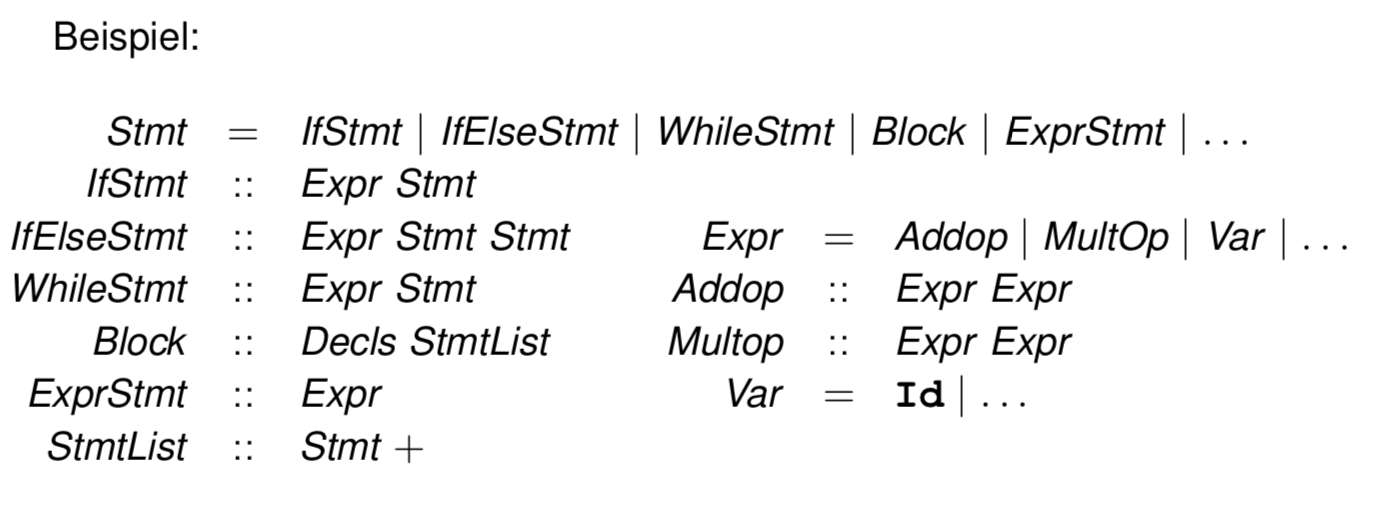
\includegraphics[width=\columnwidth]{images/abstract_syntax.png}